\subsection{A mesterséges intelligencia fogalma}
\begin{frame}{Gyenge MI vs. Erős MI}
    \begin{block}{Gyenge MI}
        \begin{itemize}
                \item Konkrét problémát old meg, de azt nagyon jól
                \item Egy konkrét algoritmussal
                \item Pl: Amazon Alexa, cicás képek azonosítása, ajánló rendszerek
            \end{itemize}
    \end{block}
    % \pause
    \centering\LARGE{$\Updownarrow$}
    % \pause
    \normalsize
    \begin{block}{Erős MI}
        \begin{itemize}
            \item Legalább olyan jól végzi el a munkát, mint az ember
            \item Általános algoritmus - {\it mindenre} jó lesz
            \item Még a közelében sem járunk
        \end{itemize}
    \end{block}
\end{frame}

\begin{frame}{Miről ismerhető fel egy szoftverben az MI?}
    \begin{itemize}
        \item<1-> A megoldandó feladat: nehéz \\
            \begin{block}{Utazó Ügynök Probléma}
                \begin{columns}
                    \begin{column}{0.5\textwidth}
                        \begin{center}
                            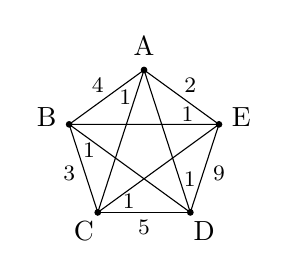
\begin{tikzpicture}
                                \foreach \x in {18,90,...,306} {
                                    \draw[fill=black,draw=black] (\x:1cm) circle [radius=1pt];
                                    \draw (\x:1cm) -- (\x+72:1cm);
                                }
                                \draw (18:1cm) -- (162:1cm)
                                      (18:1cm) -- (234:1cm)
                                      (90:1cm) -- (234:1cm)
                                      (90:1cm) -- (306:1cm)
                                      (162:1cm) -- (306:1cm);
                                \draw (90:1.3cm) node{A}
                                      (162:1.3cm) node{B}
                                      (234:1.3cm) node{C}
                                      (306:1.3cm) node{D}
                                      (18:1.3cm) node{E};
                                \draw (18+36:1cm) node{\footnotesize{2}}
                                      (90+36:1cm) node{\footnotesize{4}}
                                      (162+36:1cm) node{\footnotesize{3}}
                                      (234+36:1cm) node{\footnotesize{5}}
                                      (306+36:1cm) node{\footnotesize{9}}
                                      (18+20:0.7cm) node{\footnotesize{1}}
                                      (90+20:0.7cm) node{\footnotesize{1}}
                                      (162+20:0.7cm) node{\footnotesize{1}}
                                      (234+20:0.7cm) node{\footnotesize{1}}
                                      (306+20:0.7cm) node{\footnotesize{1}};
                            \end{tikzpicture}
                        \end{center}
                    \end{column}
                    \begin{column}{0.4\textwidth}
                        \begin{table}[h!]
                            \centering
                            \begin{tabular}{r|l}
                                Csúcs & Utak száma \\ \hline \hline
                                5 & 24 \\
                                10 & 362880 \\
                                25 & $\sim 6 \cdot 10^{23}$
                            \end{tabular}
                            % \caption{Lehetséges utak száma}
                        \end{table}
                    \end{column}
                \end{columns}
            \end{block}
        \item<2-> A szoftver viselkedése: intelligens
            \begin{itemize}
                \item Automatikus következtetés
                \item Megszerzett ismeret tárolása
            \end{itemize}
        \item<3-> Felhasznált eszközök: sajátosak
            \begin{itemize}
                \item Heurisztikával megerősített hatékony algoritmusok
                \item Gépi tanulás módszerei
            \end{itemize}
    \end{itemize}
\end{frame}
